\chapter{Grundlegende Eigenschaften}
    Übergangsmetalloxide zeigen zahlreiche und unterschiedlichste Eigenschaften wie den Ferro- oder Antiferromagnetismus~\cite{IF_5}.
    Ihr großer Variationsbereich ist Thema aktueller Forschung und soll im \autoref{sec:TMO} genauer behandelt werden.
    Eine besondere Untergruppe der Übergangsmetalloxide sind die Antiferromagneten.
    Durch die antiferromagnetische Kopplung der Lagen ergeben sich neue Phänomene, wie zum Beispiel eine hohe Magnonenfrequenz, auf die in \autoref{sec:AFM} näher eingegangen wird.
    Organisch-anorganische Grenzflächen finden heute bereits Anwendung in organischen Leuchtdioden und organischen Feldeffekttransistoren~\cite{IF_3}.
    Hierfür ist besonders die Wechselwirkung der organischen Materialien mit den anorganischen Oberflächen relevant, welche in \autoref{sec:WW} erläutert wird.
    Zudem werden in dieser Arbeit verschiedene Substrate und Oberflächenorientierungen verwendet, um das Verhalten von Pentacen-Molekülen auf den antiferromagnetischen Oberflächen zu untersuchen.
    Eine Einführung und ein Überblick über die verwendeten Systeme wird in \autoref{sec:Systeme} gegeben.

    \section{Übergangsmetalloxide} \label{sec:TMO}
        % Eine Vielzahl an Übergangsmetalloxiden kommen auf natürliche Weise in unserer Umwelt vor.
        % So ist Rost wohl ein der Bekanntesten, dabei handelt es sich um eine Form des Eisenoxids.
        % Magnetit hingegen ist in der Wissenschaft bekannt, da es das erste entdeckte magnetische Material ist~\cite{Magnetit}.
        Die magnetischen, elektronischen und geometrischen Eigenschaften der Übergangsmetalloxide variieren über einen gewissen Bereich.
        % Es gibt ferro- und antiferromagnetische Übergangsmetalloxide~\cite{IF_5}.
        Ihre elektrische Leitfähigkeit reicht von hochtemperatursupraleitend über leitend und halbmetallisch bis hin zu isolierend~\cite{IF_5}.
        Eine flächenzentrierte Struktur wie auch die Spinellstruktur wird für einige Oxide eingenommen, die auf demselben Übergangsmetall beruhen~\cite{FeO_26}.
        Aufgrund ihrer vielfältigen elektrischen Eigenschaften sowie ihrer einfachen Herstellung eignen sie sich für die Anwendung, was die Übergangsmetalloxide in den letzten Jahren zunehmend in den Fokus der aktuellen Forschung gerückt hat~\cite{IF_6, parkinson_iron_2016, cornell_iron_2003}.
        Heutzutage finden die Übergangsmetalloxide bereits ihren Einsatz im Bereich der organisch-anorganischen Grenzflächen, um den Kontaktwiderstand zu verringern, was durch die Anpassung der Austrittsarbeit gelingt~\cite{IF_11, NiO_40}.
        % Ferner werden sie schon heute zum Beispiel in organischen Transistoren, Solarzellen, Magnetstreifen und LEDs eingesetzt~\cite{IF_3}.

        Übergangsmetalloxide bestehen aus einem Übergangsmetall dem Kation und Sauerstoffatomen als Anionen.
        Bei Monooxiden, wie dem Nickeloxid (\ce{NiO}) und Wüstit (\ce{FeO}), nehmen die Übergangsmetallionen eine oktaedrische Position zwischen den Sauerstoffionen ein.
        Ihre Eigenschaften werden maßgeblich durch den Überlapp der beteiligten Orbitale bestimmt~\cite{kupper_electronic_2005}.
        Bei der Bindung zwischen dem Sauerstoff p-Orbital und dem Übergangsmetall s-Orbital kommt es zur Hybridisierung und Ausbildung neuer Zustände.
        Durch die Bindung fallen die s-Orbital-Elektronen des Metalls bei der Ladungsabschirmung der d-Elektronen weg, was in Folge der stärkeren Elektron-Elektron-Wechselwirkung zu einer stärkeren Lokalisierung der beteiligten Elektronen führt~\cite{dane_beschreibung_2008}.
        In Anwesenheit des Kristallfeldes der Liganden spalten die entarteten Zustände auf.
        In einem oktaedrischen Kristallfeld werden die Orbitale $d_{z^2}$ und $d_{x^2-y^2}$ energetisch angehoben und die Anderen energetisch abgesenkt.
        Die neuen Energieniveaus zeigen durch die Wechselwirkung zwischen Ladung, Orbitalen, Gitter und Spin magnetische Eigenschaften.
        So ergeben sich \textit{High}- und \textit{Low}-Spin Zustände, bei denen der größte (kleinste) möglichste Gesamtspin durch die Besetzung der Energieniveaus mit gleichen (entgegengesetzten) Spins erreicht wird.
        % In Folge dessen sind sie abhängig von den Oxidationszuständen, der Stöchiometrie und der Struktur.

        \begin{figure}
            \centering
            \begin{subfigure}{0.48\textwidth}
                \centering
                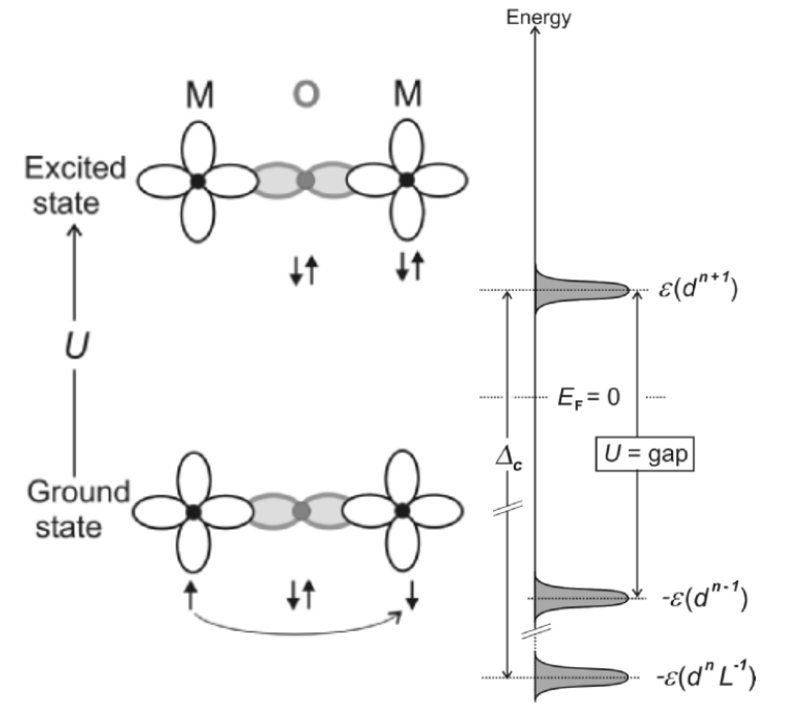
\includegraphics[height=5cm]{Mott_mod.pdf}
                \subcaption{}
                \label{fig:Mott}
            \end{subfigure}
            \begin{subfigure}{0.48\textwidth}
                \centering
                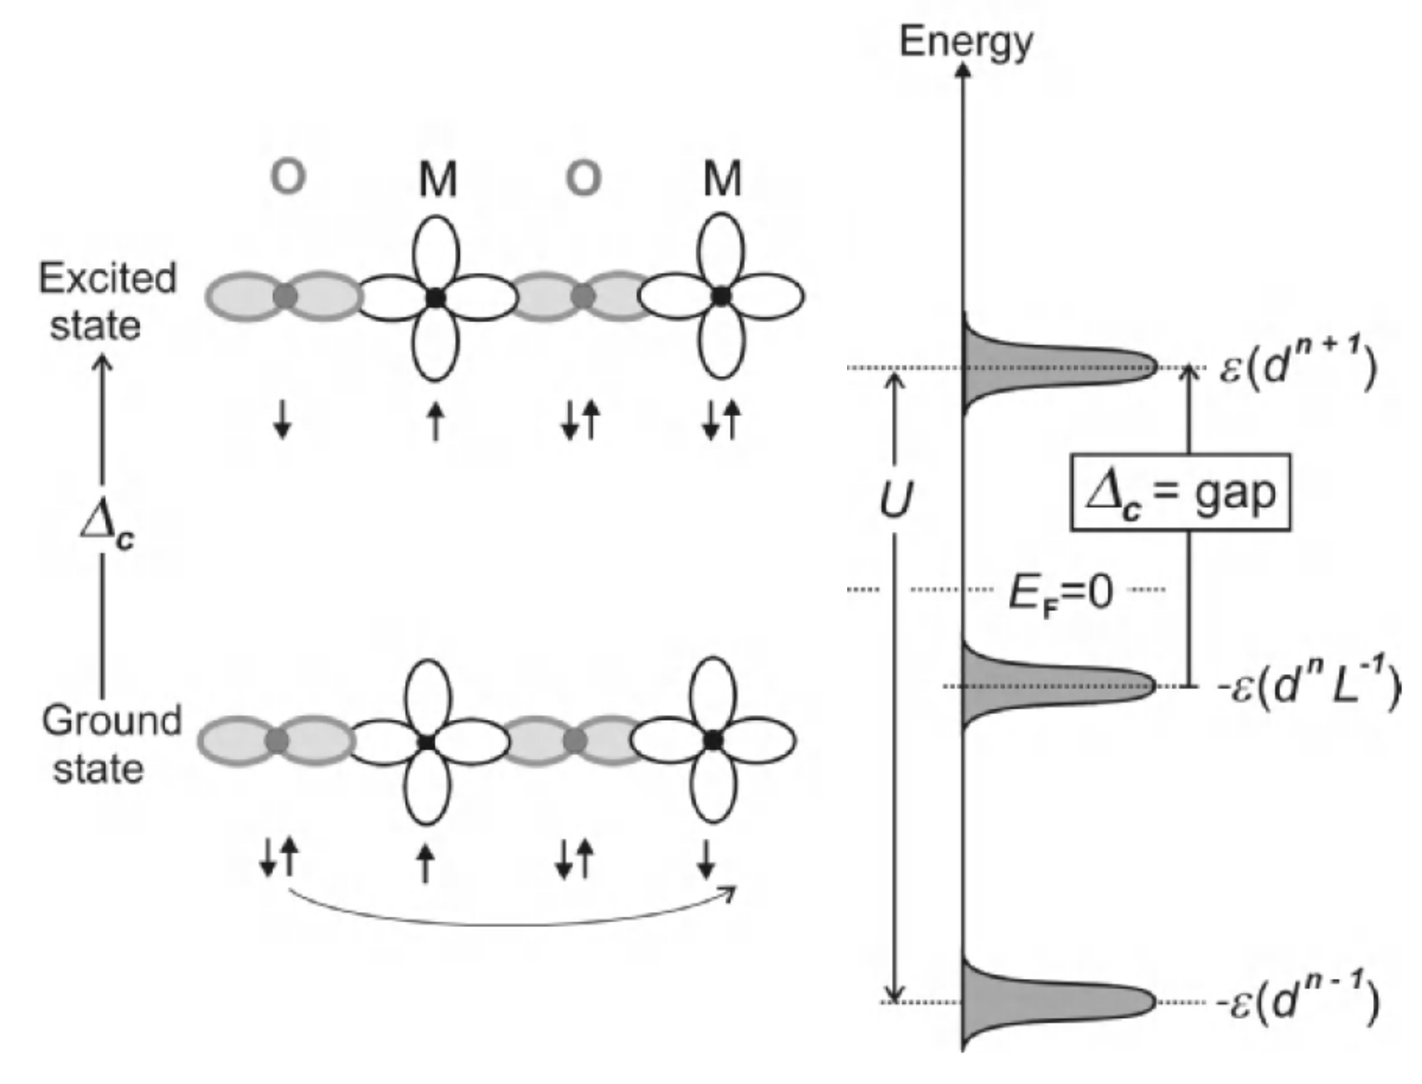
\includegraphics[height=5cm]{Charge_mod.pdf}
                \subcaption{}
                \label{fig:Charge}
            \end{subfigure}
            \caption{Schematische Darstellung des Mott-Hubbard-Isolators (\subref{fig:Mott}) und des Ladungs-Transferisolators (\subref{fig:Charge}).
            Dabei befindet sich links im Bild die Abbildung im Realraum, wohingegen rechts die Abbildung im Raum der Zustandsdichte dargestellt ist.
            Entnommen und angepasst aus \cite{stohr_magnetism_2006}.}
            \label{fig:Bandl}
        \end{figure}
        Bei den isolierenden Übergangsmetalloxiden können sich zwei Arten von Isolatoren ausbilden, welche in \autoref{fig:Bandl} abgebildet sind.
        Entscheidend für die Art der Ausbildung der isolierenden Eigenschaft ist das Verhältnis zwischen der Austauschwechselwirkungsenergie~$U$ und der Ladungsübertragsenergie~$\Delta$.
        Durch die Austauschwechselwirkungsenergie~$U$ wird der Energieaufwand beschrieben, der notwendig ist, um ein Elektron von einem Metallatom zu entfernen und es zu einem weiteren Metallatom hinzuzufügen.
        Die Energie, die aufgewendet wird, um ein Elektron von einem Liganden zum Metall zu übertragen, wird als Ladungsübertragsenergie~$\Delta$ bezeichnet~\cite{stohr_magnetism_2006}.
        Ist $\Delta$ größer als $U$ so wandert ein Elektron aus dem Grundzustand durch die Anregung von einem Metallatom zum Nächsten.
        Hierbei handelt es sich um Mott-Hubbard-Isolatoren, die Bandlücke wird durch $U$ definiert.
        Gilt im Gegensatz dazu $\Delta < U$, handelt es sich um Ladungstransfer-Isolatoren.
        Eine Anregung sorgt dafür, dass ein Elektron eines Liganden im Grundzustand zu einem Metallatom übertragen wird.
        Die Bandlücke wird durch $\Delta$ beschrieben.
        Zu letzteren zählen das Nickeloxid und Wüstit, welche trotz teilweise gefüllten d-Bändern Isolatoren sind~\cite{IF_5}.

        Im Gegensatz zu volumenkristallinen Eigenschaften sind die Eigenschaften von dünnen Filmen und Oberflächen bislang wenig erforscht.
        % Dünne Filme von einigen Monolagen aus Übergangsmetalloxiden stellen einen Teilbereich der Festkörperphysik dar und bringen durch ihre zusätzliche Einschränkung neue Möglichkeiten mit sich.
        So lässt sich im Fall von Eisenoxid ein dünner Film von Magnetit (\ce{Fe3O4}) durch Heizen in Wüstit (\ce{FeO}) überführen~\cite{FeO_1} oder durch Ionen induziertes Zerstäuben aus Hämatit (\ce{Fe2O3}) gewinnen~\cite{FeO_36}.
        Die chemischen und elektrochemischen Eigenschaften der Filme hängen maßgeblich vom Präparationsprozess ab und können zu unterschiedlichen Ergebnissen und damit Eigenschaften führen~\cite{Uni-Tübingen}.
        Durch gezieltes Eingreifen in den Präparationsprozess, z.B. durch Variation des Verhältnisses aus Sauerstoffdruck und Aufdampfrate, lässt sich die Stöchiometrie variieren.
        Eine Veränderung der Austrittsarbeit lässt sich durch Anpassung des Oxidationszustands oder durch das Einbringen von Defekten erzielen.
        Die Austrittsarbeit ist ein entscheidender Parameter bei der Energieniveauanpassung zwischen Substrat und Molekülen, infolge dessen es zu einem einfachen Ladungstransfer kommen kann (siehe \autoref{sec:ENA})~\cite{IF_3}.

        Wichtig für die Interaktion mit Adsorbaten ist die Oberfläche der Übergangsmetalloxide.
        An der Oberfläche spielen die Polarität, Anzahl ungesättigter Bindungen wie auch Defekte eine entscheidende Rolle bei der Oberflächenrekonstruktion und Reaktivität.
        Die Oberflächen der hier betrachteten 3d-Übergangsmetalloxide kristallisieren in der Kochsalzstruktur und bilden einerseits eine stabile (100)-Oberfläche als auch eine instabile (111)-Oberfläche aus.
        Dies liegt an der polaren Oberfläche der (111)-Orientierung und des damit verbundenen großen Oberflächendipolmoments.
        Hierdurch wird eine größere Reaktivität der Oberfläche erwartet~\cite{cappus_hydroxyl_1993}.
        % Anzumerken bleibt, dass dabei die Sauerstoff terminierte Oberfläche stabiler als die metallisch terminierte Oberfläche ist.
        % Ursache ist die einfachere Polarisation des Sauerstoffatoms, was das Oberflächendipolmoment reduzieren kann~\cite{al-abadleh_oxide_2003}.
        Solche reaktiven Oberflächen, meist aus dünnen Filmen, werden heute bereits zur Katalyse eingesetzt.
    
    \section{Antiferromagnetismus} \label{sec:AFM}
        Antiferromagneten (AFM) zeichnen sich dadurch aus, dass sie nach außen hin kein permanentes magnetisches Moment aufweisen.
        Vereinfacht dargestellt haben im Inneren die magnetischen benachbarten Momente den gleichen Betrag und sind antiparallel zueinander ausgerichtet~\cite{Suter}.
        Sind die beiden koppelnden magnetischen Momente nicht gleich groß, so tritt Ferrimagnetismus auf.
        Die entgegengesetzten magnetischen Momente heben sich dabei nicht auf und es ergibt sich eine makroskopische Magnetisierung.
        Dieser Zustand ist allerdings nur unterhalb der Néel-Temperatur $T_\text{N}$ stabil.
        Oberhalb verhalten sich die Antiferromagneten paramagnetisch.
        Die inneren magnetischen Momente richten sich parallel zu einem äußeren Feld aus und verstärken es somit.
        % Um das Phänomen des Antiferromagnetismus zu erklären, bedarf es der quantenmechanischen Beschreibung, unter Beachtung des Pauli Verbots und der Hundschen Regeln~\cite{TUChemnitz}.
        % Es ergibt sich der Austauschwechselwirkungshamiltonien $H_\text{A} = - J_{ik} \vec{S_i}\cdot\vec{S_k}$, welcher die direkte Wechselwirkung der Spins berücksichtigt.
        % $J_{ik}$ spiegelt dabei die Stärke der Austauschwechselwirkung wieder und folgt aus dem Überlapp der Wellenfunktionen der beteiligten Elektronen.
        % Für $J_{ik} < 0$ ergibt sich die antiferromagnetische Kopplung und für $J_{ik} > 0$ eine ferromagnetische Kopplung.
        % Um eine Aussage über die Ordnung im Antiferromagneten zu treffen, gibt es den Ordnungsparameter $L = S^{\uparrow} - S^{\downarrow}$.
        % Hierbei sind $S^{\uparrow}$ beziehungsweise $S^{\downarrow}$ der Spin der jeweiligen Untergitter.

        \begin{figure}
            \centering
            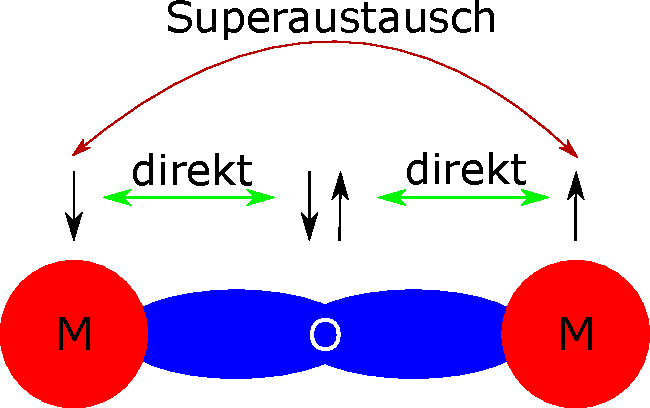
\includegraphics[width=0.6\textwidth]{AFM.pdf}
            \caption{Schematische Darstellung der antiferromagnetischen Kopplung.
            Als Ligand fungiert hier ein Sauerstoffatom mit seinem p-Orbital (blau).
            Die Spins der d-Orbitale der Metalle (rot) koppeln ferromagnetische mit denen des Sauerstoffs.
            So entsteht eine indirekte antiferromagnetische Kopplung der beiden Metallatome.}
            \label{fig:AFM}
        \end{figure}
        Bei der zugrundeliegenden Wechselwirkung im Antiferromagneten handelt es sich um den Superaustausch.
        Dabei koppeln zwei Atome mit einem magnetischen Moment über ein weiteres nicht magnetische Atom. 
        % Dabei kann die Kopplung ferro- oder antiferromagnetisch sein, meist jedoch antiferromagnetisch~\cite{AFM_1}.
        Im Allgemeinen ist der Superaustausch winkelabhängig, da der Überlapp der Orbitale entscheidend ist.
        Für die Erklärung wird sich hier allerdings nur auf die \SI{180}{\degree}-Wechselwirkung beschränkt, welche in \autoref{fig:AFM} dargestellt ist.
        Es kommt hierbei nicht zu einem Überlapp der Spin tragenden Wellenfunktionen zweier Metallatome (rot), sondern zu der Vermittlung der langreichweitigen Ordnung über einen Liganden (blau), dem indirekten Austausch.
        
        Der direkte Austausch sorgt für ferromagnetische Kopplung zweier benachbarter Spins.
        Zwischen Metall und Ligand herrscht eine direkte Austauschwechselwirkung und ihre Spins richten sich parallel zueinander aus.
        Da das koppelnde, nicht metallische Orbital voll ist, müssen die Elektronen unterschiedliche Spinausrichtung haben.
        Damit besitzt das vermittelnde Atom kein eigenes magnetisches Moment und das sich auf der anderen Seite befindende Metallatom richtet den Spin seines Elektrons parallel zu dem zweiten Spin des vermittelnden Atoms aus.
        Somit ist der Spin antiparallel zu dem des ersten Metallatoms, somit ist die Wechselwirkung über das vermittelnde Atom hinweg antiferromagnetisch. 
        Jedes der Metallatome gehört dabei einem von zwei Untergittern an, welche entgegengesetzte Spinausrichtung besitzen.
        Folglich ist die Gesamtmagnetisierung für Antiferromagneten null.
        Bei den vorliegenden Übergangsmetalloxiden sind die koppelnden Orbitale die metallischen nicht vollständig besetzten 3d-Orbitale der Übergangsmetalle und die 2p-Orbitale des Sauerstoffs.
        % Die Wellenfunktionen der Kationen überlappen nur gering und da die Austauschwechselwirkung nur geringe Reichweiten hat können nur die 3d und 2p überlappen.
        % Anwendungen finden Antiferromagneten zum Beispiel als \textit{Pinning}-Lage, die in spinelektronischen Bauteilen die Orientierung einer ferromagnetischen Schicht festlegen.
        
    \section{Wechselwirkung von Oberfläche mit Molekülen} \label{sec:WW}
        Moleküle haben im Gegensatz zu Festkörpern energetisch separierte Zustände, die Orbitale.
        Kommen die Moleküle in Kontakt mit einer Oberfläche, führt die Wechselwirkung zwischen beiden zu einer Veränderung in ihrer elektronischen Struktur.
        Dabei wird in zwei Stärken der Adsorption unterschieden.
        Die schwächere Adsorption ist die Physisorption und die stärkere die Chemisorption. % , welche wiederum in stark und schwach unterschieden wird.
        Zwischen den beiden Adsorptionsarten lässt sich durch ihre Bindungsstärke zum Substrat hin unterscheiden.
        Dabei wird als Bindungsstärke die Energie bezeichnet, die nötig ist, um ein Molekül von der Oberfläche zu lösen.
        %~\cite{ma-DJ
        
        \subsection{Physisorption}
            Bei der Physisorption existiert nur eine geringe Bindungsenergie zwischen Molekül und Substrat~\cite{IF_16}. 
            Durch die schwache Wechselwirkung der Physisorption werden die Eigenschaften der Oberfläche und des Moleküls nur schwach beeinflusst~\cite{bergenti_spinterface_2019}.
            Die Eigenschaften der Moleküle haben eine starke Ähnlichkeit zu den Eigenschaften aus der Gasphase~\cite{IF_16}.

            Bei der Physisorption ist die Van-der-Waals-Kraft maßgeblich für die Bindung verantwortlich.
            Die Van-der-Waals-Kraft gehört zu den elektrostatischen Kräften, bei der keine Elektronen mit dem Substrat ausgetauscht werden~\cite{bergenti_spinterface_2019}.
            Allein die Induzierung und Fluktuation von Dipolen führt zu einer Bindung zwischen Molekül und Substrat.
            Vermehrt tritt die Physisorption bei Halbleitern und Isolatoren auf, da die Molekülzustände in der Bandlücke liegen und so keine Bindung mit dem Substrat eingegangen werden kann~\cite{IF_1}.
            % Allerdings kann es beim Substrat zu geometrischen Spannungen kommen, infolge es zur Umstrukturierung der Atompositionen kommen kann.
            % Charakteristisch für die Physisorption ist die Abwesenheit von chemischen Bindungen.
            %, sowie einen Substrat-Adsorbat-Abstand von mehr als \SI{3}{\angstrom}. %~\cite{bergenti_spinterface_2019}
            % Die Van-der-Waals-Kraft kann man in drei Arten unterteilen:
            % \begin{itemize}
            %     \item \textbf{Dipol-Dipol-Kraft:} Sie ist die Kraft zwischen zwei permanenten Dipolen, die Keeson-Wechselwirkung.
            %     \item \textbf{Dipol-induzierter-Dipol-Kraft:} Die Wechselwirkung zwischen einem induziertem Dipol und einem Dipol wird auch als Debye-Wechselwirkung bezeichnet.
            %     \item \textbf{Londonsche Dispersions-Wechselwirkung:} Zwischen zwei induzierten Dipolen wirkt die Londonsche Dispersions-Wechselwirkung, sie dominiert meist die Van-der-Waals Kraft.
            % \end{itemize}
            % Die Physisorption kann durch das Lennard-Jones-Potential beschrieben werden.
            % Es setzt sich dabei aus dem repulsiven Potential und dem Potential der Debye-Wechselwirkung zusammen.
            % Der repulsive Anteil resultiert aus dem Pauliverbot. 
            % Kommen sich Molekülorbital und Substratorbital zu nah, überlappen diese.
            % Auf Grund des Pauliverbots dürfen sich keine zwei Elektronen in allen Quantenzahlen gleichen und es resultiert in einer abstoßenden Kraft.
            % Durch die attraktive Anziehung aus der Debye-Wechselwirkung führt beim Gleichgewicht dies zu einem stabilen Substrat-Molekül-Abstand.
        
        \subsection{Chemisorption}
            Im Gegensatz zur Physisorption sind die Bindungen bei der Chemisorption um einiges stärker und führen somit zu Veränderung an der chemischen sowie elektronischen Struktur des Substrats wie auch der Moleküle~\cite{bergenti_spinterface_2019}.
            Ferner wird von Chemisorption gesprochen, wenn die Stärke der Wechselwirkung größer als \SI{1}{\electronvolt} ist~\cite{muscat_chemisorption_1978} und eine chemische Bindung auftritt.
            Dabei kann es sich um kovalente und ionische Bindungen handeln, welche einen Ladungsaustausch und/oder Hybridisierung begünstigen~\cite{harutyunyan_hybridisation_2013}.
            Beim Ladungsaustausch kann ein zunächst unbesetztes Orbital unter die Fermikante fallen und besetzt werden.
            Im Gegensatz dazu können bei der Hybridisierung mehrere Zustände vom Molekül und/oder Oberfläche durchmischt werden und so zu Verbreiterungen, Verschiebungen und Aufspaltungen von Molekülzuständen führen~\cite{IF_1}.
            
            Die Chemisorption wird weiter in eine schwache und starke Adsorption unterschieden.
            Schwache Bindungen werden meist durch die Wechselwirkung mit den breiten s- oder p-Bändern hervorgerufen, wodurch sich das Energieniveau der Moleküle absenkt und verbreitert (Schritt (1) in \autoref{fig:Chemisorption} oben).
            \begin{figure}
                \centering
                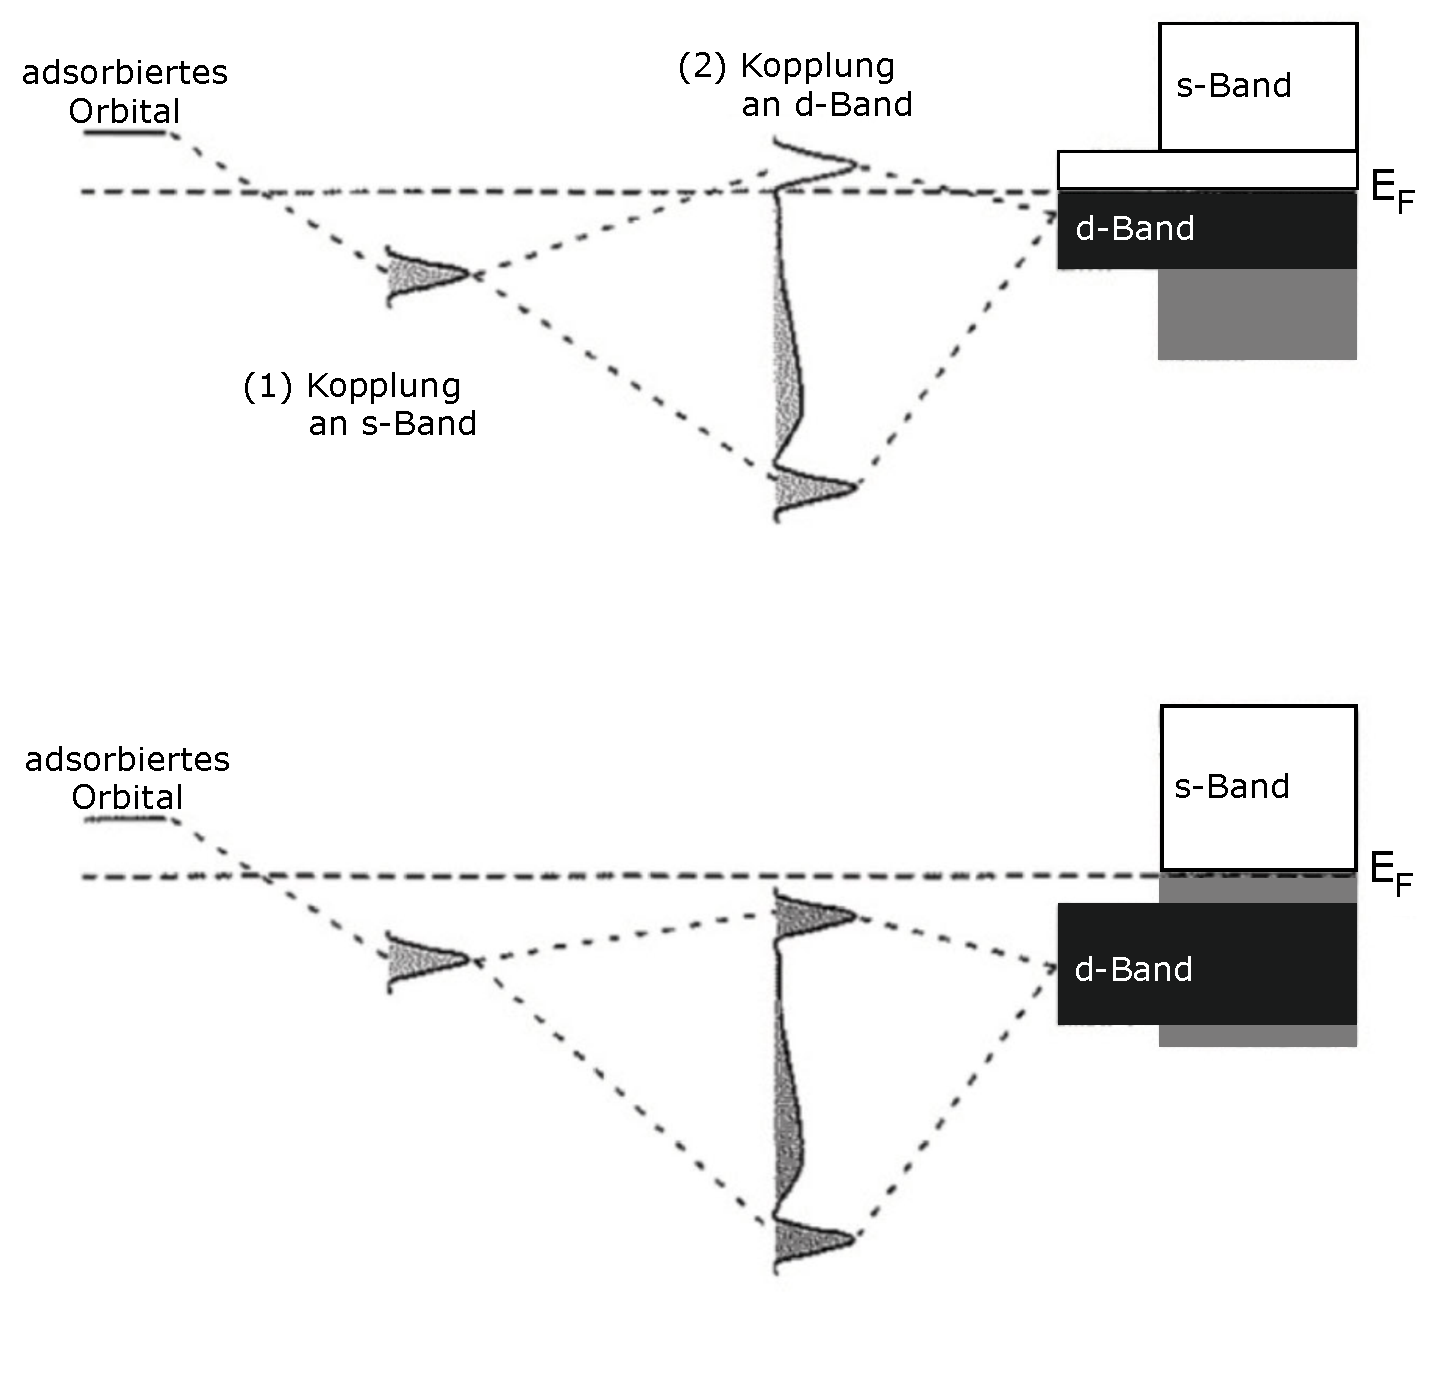
\includegraphics[width=0.5\textwidth]{Chemisorption.pdf}
                \caption{Adsorbierte Moleküle hybridisieren mit den s/p-Band des Substrates (1).
                Anschließend koppelt dieser Zustand mit den d-Bändern (2).
                Eine starke Chemisorption oben und schwache Chemisorption unten.
                Entnommen aus~\cite{IF_1} und modifiziert.}
                \label{fig:Chemisorption}
            \end{figure}
            Bei der starken Chemisorption überlappt dieser abgesenkte Zustand mit den d-Bändern und es bilden sich dabei bindende und antibindende Zustände aus (Schritt (2) in \autoref{fig:Chemisorption} oben).
            Je nach Lage des Ferminiveaus wird nur der bindende Zustand (starke Adsorption) oder (nur teilweise) der antibindende Zustand gefüllt.
            Durch die (teilweise) Füllung des antibindenden Zustands treten repulsiv Kräfte auf und die Adsorptionsstärke wird geschwächt (\autoref{fig:Chemisorption} unten).

        \subsection{Selbstanordnung} \label{sec:Selbstanordnung}
            Molekül können auf Oberflächen eine regelmäßige Überstruktur ausbilden, wenn sich Molekül-Molekül- und Molekül-Substrat-Wechselwirkung in einem richtigen Verhältnis zueinander befinden.
            Dieser Effekt wird Selbstanordnung genannt.
            Besonders für die Untersuchung der elektronischen Struktur mittels Photoemissionsorbitaltomographie (siehe \autoref{sec:MOT}) spielt dies eine große Rolle, da dafür die Moleküle einheitlich auf der Oberfläche orientiert sein müssen.
            Ferner lassen sich gitterartig verteilte Moleküle gezielter manipulieren, dass für zukünftige Anwendungen, wie etwa Datenspeicher, wichtig ist.
            
            Das Wechselspiel zwischen der Molekül-Molekül-Wechselwirkung und Molekül-Substrat-Wechselwirkung definiert die finale Struktur~\cite{IF_1}.
            Dabei sind vor allem gerichtete Kräfte wichtig, um die gewünschte Regelmäßigkeit der Überstruktur zu erhalten.
            Die schwächste und ungerichteste Kraft ist die Van-der-Waals-Kraft beziehungsweise die Debye-Wechselwirkung. % (\SIrange{0.02}{0.1}{\electronvolt}).
            Diese langreichweitige Wechselwirkung tritt immer auf und kann zu großflächigen einheitlichen Strukturen führen.
            Eine wichtige Bindung für Wasserstoff enthaltene Moleküle ist die Wasserstoff-Brücken-Bindung mit kurzen Bindungslängen. % einer Energie von \SIrange{0.01}{1.73}{\electronvolt}
            Je stärker diese Wechselwirkung, desto geradliniger wirkt sie.
            Durch metallische Atome kann es zu einer metallischen Koordination kommen und die Moleküle fungieren als Verbinder zwischen einzelnen Metallatomen. % (\SIrange{0.5}{2}{\electronvolt})
            % Weitere Ursache ist der Einfluss des Substrates auf die Wechselwirkung den Molekülen untereinander, z.B. durch Oszillationen des Oberflächenpotentials.
            Die stärkste und gerichteste Kraft ist jedoch die kovalente Bindung, welche einerseits die elektronische Struktur stark beeinflusst als auch die Selbstanordnung von Molekülen behindern kann, wodurch weniger geordneten Strukturen entstehen~\cite{IF_1}.
            % Für Moleküle mit einem permanenten Dipolmoment muss ebenfalls die Keeson-Wechselwirkung (Dipol-Dipol-Wechselwirkung) berücksichtigt werden.

            \begin{figure}
                \centering
                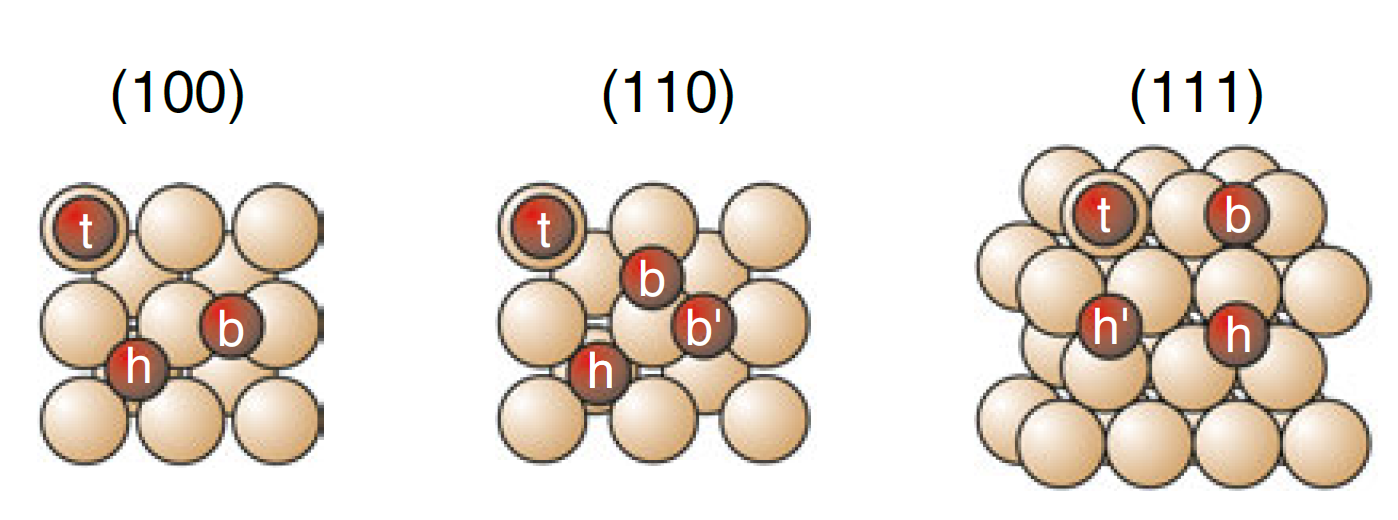
\includegraphics[width=0.6\textwidth]{Adsorbate}
                \caption{Die Adsorbatplätze für verschieden orientierte Oberflächen eines flächenzentrierten Kristalls.
                Die Plätze werden nach ihrer relativen Position zwischen Adsorbat und Substartatom benannt.
                Direkt oberhalb eines Substratatoms (\textit{on top} - t), zwischen zwei Substratatomen mit kleinem Abstand (b) und großem Abstand (b'), den Brückenplätze (\textit{bridge}).
                Sowie Muldenplätze hexagonaler dicht gepacktester Struktur (\textit{hollow} - h) und flächenzentrierter Struktur (h'). Aus~\cite{Fauster}.}
                \label{fig:Adsorbate}
            \end{figure}
            Bei der Adsorption können sich die Moleküle an drei unterschiedlichen Positionen auf dem Substrat absetzen (bezogen auf das Zentrum des Moleküls).
            Dabei wird zwischen dem Platz direkt über einem Substratatom (\textit{on top}), zwischen zwei Substratatomen (\textit{bridge}) oder in der Mitte von mehreren Substratatomen in einer Mulde (\textit{hollow}) unterschieden.
            Beispielhaft ist dies schematisch für einen flächenzentrierten Kristall mit verschiedenen Oberflächen in \autoref{fig:Adsorbate} dargestellt.
            Eine Vorhersage bei welcher Eigenschaftskombination sich Moleküle selbstanordnen und auf welchen Plätzen, kann aktuell nicht getroffen werden.
            Grund hierfür sind die zahlreichen beteiligten Wechselwirkungen und die Möglichkeit Elektronen auszutauschen. 

            \begin{figure}
                \centering
                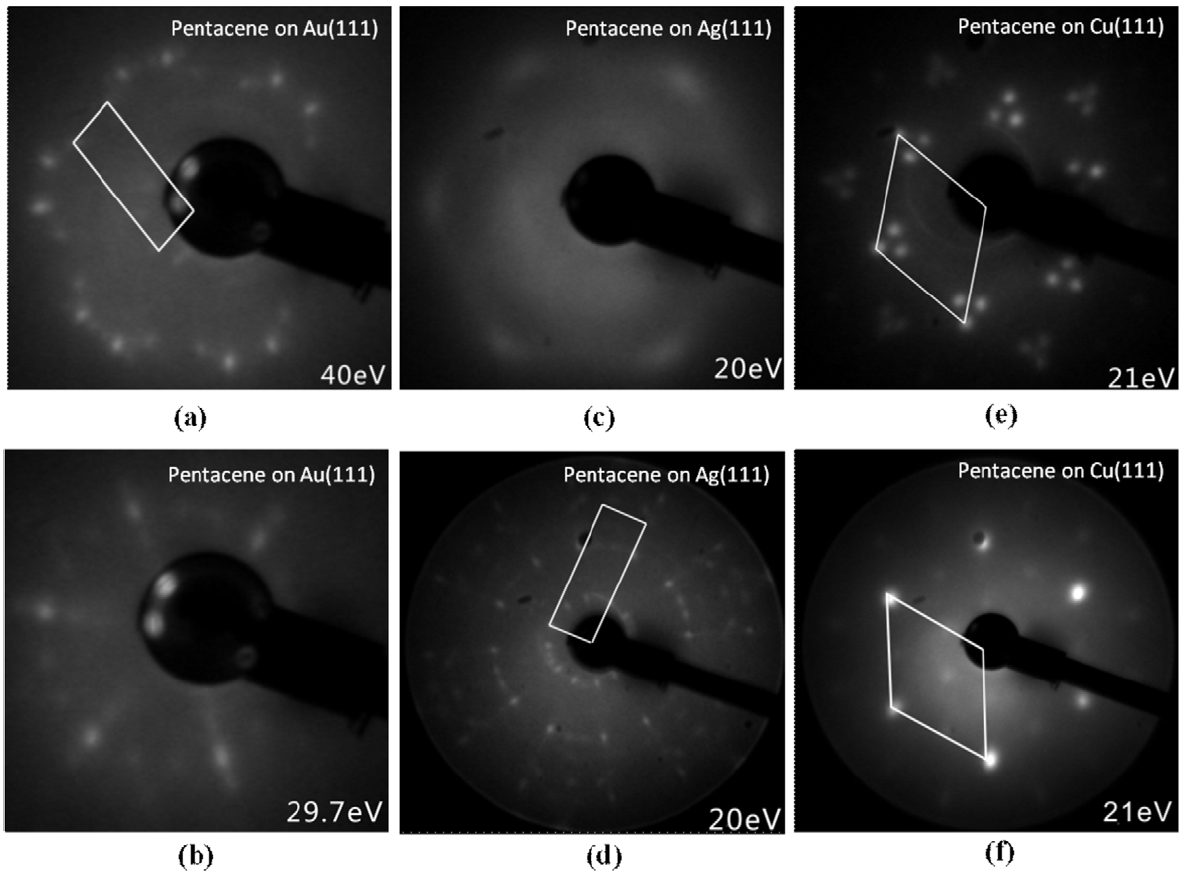
\includegraphics[width=0.6\textwidth]{PEN_Sub.PNG}
                \caption{Abgebildet sind die Aufnahmen der Beugung niederenergetischer Elektronen für verschiedene Schichtdicken von Pentacen auf der (111)-Oberfläche von Gold (a und b), Silber (c und d) und Kupfer (e und f).
                Die Bilder oben entsprechen einer Bedeckung von einer Monolage, die Bilder unten einer Bilage Pentacen.
                Kopiert aus~\cite{5A_4}.}
                \label{fig:PEN_Sub}
            \end{figure}
            Ist die Molekül-Substrat-Wechselwirkung kleiner als die Wechselwirkung zwischen den Molekülen, bilden sich vermehrt geordnete Filme, die jedoch nicht an dem Substrat ausgerichtet sind.
            Ist im Gegensatz dazu die Wechselwirkung unter den Molekülen geringer als die zum Substrat, bilden sich Filme aus, welche sich an die Geometrie des Substrates anpassen oder die Moleküle können nicht diffundieren und bleiben in einer ungeordneten Struktur.
            Mit steigender Schichtdicke nimmt die Wechselwirkung mit dem Substrat ab und die Wechselwirkung der Moleküle untereinander überwiegt, wodurch sich die Kristallstruktur der Moleküle ausbildet~\cite{5A_9}.
            Für verschiedene Substrate und Bedeckungen ergeben sich verschiedene Ordnungen auf der Oberfläche, was auf die unterschiedliche Stärke der Wechselwirkung zurückzuführen ist.
            Dass die Wechselwirkmechanismen zwischen Substrat und Molekül eine entscheidende Rolle darstellen, lässt sich am Beispiel von Au(111) (Physisorption),  Ag(111) (schwache Chemisorption) und Cu(111) (starke Chemisorption) in Kombination mit verschiedenen Schichtdicken von Pentacen Molekülen in \autoref{fig:PEN_Sub} erkennen~\cite{5A_4}.
            Ebenfalls sichtbar ist, dass die Schichtdicke einen wichtigen Faktor bei der Selbstanordnung darstellt.
            Ein weiterer Einfluss ist die Diffusion der Moleküle, welche maßgeblich durch die Oberflächenbeschaffenheit und Temperatur behindert werden kann.
            Ist die Aufdampfrate zu groß für die Diffusionsrate, bilden die Moleküle keine wohldefinierte Struktur aus~\cite{IF_15}.            

        \subsection{Energieniveauanpassung} \label{sec:ENA}
            Für die Anwendung ist die Energieniveauanpassung besonders bedeutsam, da sie Einfluss auf den Elektronen- und Lochtransport hat~\cite{IF_4}.
            Bei Metalloxiden verschiebt sich durch die Austrittsarbeit $\phi$ die relative Position des Valenz- und Leitungsbandes zum Vakuumniveau~\cite{IF_3}.
            Die meisten Isolatoren haben keine besetzten Zustände nahe der Fermikante, da diese in eine Bandlücke fällt.
            Folglich ist auch ein Ladungsübertrag vom Substrat auf die Moleküle nur vom Valenz- oder Leitungsband aus möglich.
            Dies unterscheidet den Prozess maßgeblich von vielen Modellen für Metall-organischen Grenzflächen.
            Auch wenn einige Oxide Ladungsaustausch zwischen Valenzband und dem höchsten besetzten Molekülorbital (HOMO, \textit{highest occoupied molecular orbital}) zulassen, existiert noch kein Model, dass dies beschreibt~\cite{IF_3}.
            Wichtig für den Ladungsaustausch sind Donator- und Akzeptorzustände der Moleküle und des Substartes.
            Dabei gilt das HOMO als der Molekül-Donator-Zustand und das LUMO (niedrigstes unbesetztes Molekülorbital, \textit{lowest unoccoupied molecular orbital}) als Akzeptor-Zustand.
            Bei den Übergangsmetalloxiden gilt das Leitungsband als Akzeptorzustand und das Valenzband als Donatorzustand. 
            
            Verbreitet ist der Ansatz der Ferminiveau-Anheftung für nichtreaktive Grenzflächen zwischen den Molekülen und den Oxiden.
            Greiner u.a.~\cite{IF_3} fanden heraus, dass die Bandstruktur des Substrates dabei nur eine untergeordnete Rolle spielt.
            \begin{figure}
                \centering
                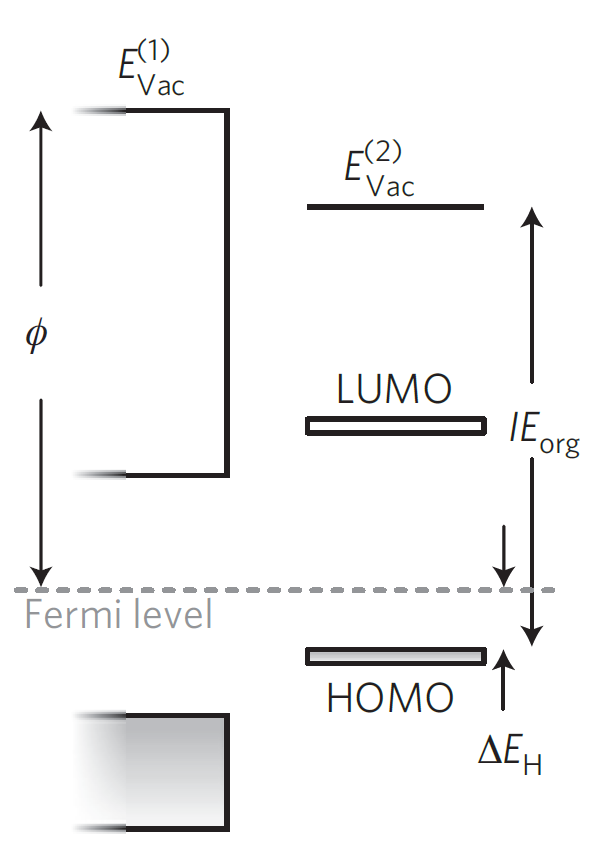
\includegraphics[height=6cm]{E_align.PNG}
                \caption{Schema für die Energieniveauanpassung zwischen dem Übergangsmetalloxid und den Molekülen. Kopiert aus~\cite{IF_3}.}
                \label{fig:E_align}
            \end{figure}
            Ausschlaggebend für die Energieniveauanpassung ist das elektrochemische Potential des Substrates mit dem Reduktionspotential des Moleküls, genauer die Differenz zwischen der Austrittsarbeit des Substrates und der Ionisationsenergie $IE_\text{org}$ des Moleküls (siehe \autoref{fig:E_align}).
            Als Ionisationsenergie wird die Energie zwischen dem höchsten besetzten Molekülorbital und dem Vakuumniveau verstanden.
            Der Energie-Offset $\Delta E_\text{H}$ beschreibt die Energiedifferenz zwischen HOMO und Fermikante des Substrates.
            Die Austrittsarbeit eines Substrates ist dabei umso kleiner, je reaktiver es ist~\cite{5A_5}.
            Steigt die Austrittsarbeit des Substrates über die Ionisationsenergie des Moleküls, so wird die Bindungsenergie des Molekülorbitals für steigende Austrittsarbeiten auf einem konstanten Wert gehalten.
            Somit wird das HOMO mit einer gewissen Bindungsenergie an das Fermilevel angeheftet, die nur von der Differenz zwischen der Austrittsarbeit und des Ionisationspotential abhängt.
            Sinkt hingegen die Austrittsarbeit unter die Ionisationsenergie, steigt der Energie-Offset an.
            Der ganze Prozess der Ausrichtung der Molekülzustände an das Ferminiveau des Substrates wird Ferminiveau-Anheftung genannt~\cite{IF_3}.
            Als Folge des Energieniveauanpassung und dem möglichen Ladungsaustausch oder Hybridisierung kommt es zur Verkürzung der Lebenszeit der Molekülorbitale.

            Das zusätzliche Auftreten eines Oberflächendipolmoments hat Einfluss auf die Austrittsarbeit und damit auf die Ferminiveau-Anheftung.
            Durch eine Verschiebung von Ladungsträgern kann sich das Oberflächendipolmoment weiter ausbilden und damit die Austrittsarbeit verringern~\cite{5A_5}.
            Wegen des Pauliverbots und den zusätzlichen Elektronen der Moleküle an der Grenzfläche werden die Elektronen an der Oberfläche in den Festkörper zurückgedrängt.
            Durch die Unabhängigkeit vom Adsorptionstyp tritt dieser \textit{Push-Back}-Effekt immer auf~\cite{IF_4} und reduziert damit das Oberflächendipolmoment~\cite{IF_1}.
            Zusätzlich kann das Oberflächendipolmoment durch Ladungsaustausch zwischen Molekül und Substrat geschwächt oder gestärkt werden.
            % Hinzukommend gibt es gegebenen falls noch einen permanenten Dipol des Moleküls, welcher beachtet werden muss.
            % Weiter gehend ist zu beachten, dass auch bei Isolatoren sich ein Oberflächendipol ausbilden kann.

    \section{Systemeigenschaften} \label{sec:Systeme}
        Entscheidend für alle Prozesse ist die Wahl des Substrates und der verwendeten Moleküle.
        In dieser Arbeit wurden zwei unterschiedliche Substrate gewählt, das Nickeloxid (111) und das Eisenmonooxid (100).
        Beide zeigen isolierende Eigenschaften und kristallisieren in der \ce{NaCl}-Struktur.
        Die Wahl der \ce{NiO}(111)-Oberfläche ist durch die erwartete höhere Reaktivität aufgrund der polaren Oberfläche~\cite{cappus_hydroxyl_1993} und der gleichgerichteten Spins begründet.
        % Das Nickeloxidsubstrat weist eine (111)-orientierte Oberfläche auf in der die Spins an der Oberfläche alle in dieselbe Richtung zeigen.
        % Auch stellt diese Orientierung eine erhöhte Reaktivität im Gegensatz zu anderen Orientierungen da~\cite{cappus_hydroxyl_1993}. % und ist durch die vermutete höhere Reaktivität begründet.
        Um Wüstit zu erhalten wird, zunächst Magnetit als Ausgangsmaterial verwendet und durch mehrere Präparationsprozesse in das gewünschte Wüstit umgewandelt.
        Die (100)-orientierte Oberfläche des Wüstits sollte eine geringere Reaktivität als die (111)-orientierte Oberfläche zeigen, des Weiteren sind auf ihr die Spins der Eisenionen abwechselnd gerichtet. % ist aufgrund der geordneten Struktur ein geeignetes Material für das Wachstum von Molekülen.
        \begin{table}
    \centering
    \caption{Zusammenfassung der wichtigsten Systemparameter der verwendeten Substrate.}
    \label{tab:Systeme}
    \begin{tabular}{l c c}
        \toprule
        {Materialeigenschaften} & {NiO} & {FeO} \\
        \midrule
        Kristallstruktur \cite{sebbari_uranyl_2012} & \ce{NaCl} & \ce{NaCl} \\
        Gitterkonstante & \SI{4.17}{\angstrom} \cite{sebbari_uranyl_2012} & \SI{4.308}{\angstrom} \cite{springer_database}\\
        Oberflächenorientierung & (111) & (100) \\
        % \multirow{2}{*}{Oberflächenrekonstruktion \footnote{bzgl. des Substartes}} & Domänen (100) & $\text{p}(1 \times 1)$ inv. Intensitäten\\
        % & & \\
        magn. Eigenschaft \cite{FeO_6}& antiferromagnetisch & antiferromagnetisch \\
        Neèl-Temperatur \cite{FeO_6} & \SI{525}{\kelvin} & \SI{198}{\kelvin} \\
        Austrittsarbeit & \SIrange{4.5}{5.2}{\electronvolt} \cite{poulain_electronic_2020} & \SI{3.5}{\electronvolt} \cite{FeO_28}\\
        Bandlücke & \SI{3.6}{\electronvolt} \cite{kunz_chemisorption_1985} & \SI{2.4}{\electronvolt} \cite{FeO_21}\\
        \bottomrule
    \end{tabular}
    
\end{table}

        Eine Übersicht über die wichtigsten Systemparameter ist in \autoref{tab:Systeme} gegeben.
        Ein kleines Molekül für das auf vielen Oberflächen Selbstanordnung initiiert werden kann und bereits als organischen Halbleiter eingesetzt wird, ist das Pentacen~\cite{5A_9, 5A_13}.

        \subsection{Nickeloxid} \label{sec:NiO}
            Die Struktur des Nickeloxids ist in \autoref{fig:NiO-structure} dargestellt~\cite{kunz_chemisorption_1985}.
            \begin{figure}
                \centering
                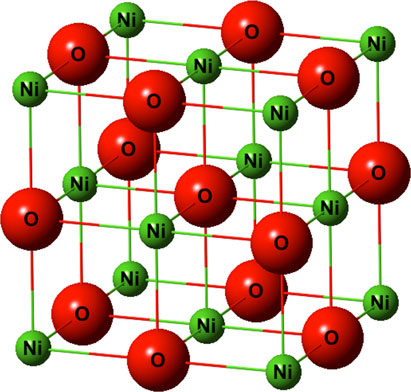
\includegraphics[height=5cm]{NiO/NiO-structure.jpg}
                \caption{Kristallstruktur von Nickeloxid.
                Das $\ce{Ni}^{2+}$-Ion befindet sich in einer oktaedrischen Umgebung von $\ce{O}^{2-}$-Ionen.
                Entnommen aus ~\cite{NiO-structure}.}
                \label{fig:NiO-structure}
            \end{figure}
            Hierbei handelt es sich um ein Monooxid, beidem die Sauerstoffatome in den oktaedrischen Zwischenräumen zwischen den Nickelatomen sitzen.
            Die geometrische Gitterkonstante beträgt \SI{4.17}{\angstrom}~\cite{sebbari_uranyl_2012}, wohingegen sich für die magnetische Ordnung die doppelte Gitterkonstante zwischen zwei gleich ausgerichteten Spins ergibt~\cite{Suter}.
            Die Spins innerhalb einer (111)-Ebene koppeln ferromagnetisch, wohingegen die Kopplung unter den Ebenen antiferromagnetisch ist~\cite{FeO_6}.
            Somit gehört Nickeloxid zu der Familie der Antiferromagneten, mit einer Neél-Temperatur von \SI{525}{\kelvin}~\cite{FeO_6}.

            Das 3d-Band des Nickeloxids ist mit nur acht von zehn möglichen Elektronen besetzt und dennoch ein Ladungstransfer-Isolator mit einer Bandlücke von \SI{3.6}{\electronvolt}~\cite{kunz_chemisorption_1985}.
            Die Austrittsarbeit lässt sich durch die Präparation beeinflussen und liegt zwischen \SIrange[range-phrase=\:und\:]{4.5}{5.2}{\electronvolt}~\cite{poulain_electronic_2020}.

            Das Oberflächendipolmoment ist besonders stark in der (111)-Orientierung ausgeprägt, da bei der polaren Oberfläche entweder nur Sauerstoff- oder nur Nickelionen in der obersten Lage vorhanden sind~\cite{NiO_8}.
            Das Oberflächenpotential ist folglich divergent und somit die Oberfläche instabil.
            Problematisch an dünnen Filmen von Nickeloxid in der (111)-Orientierung ist dessen Instabilität und die Abhängigkeit von den Präparationsparametern~\cite{NiO_36}.
            Es gibt verschiedene Beobachtungen zur Stabilisierung der polaren Oberfläche wie Rekonstruktionen oder eine \ce{OH-}-Terminierung~\cite{NiO_36, NiO_35, NiO_34, NiO_27, NiO_10}.
            Bei der Stabilisierung wird die Oberflächenladung reduziert und in Folge dessen kann es zur Ausbildung einer stabilen Oberfläche kommen.
            % Hinsichtlich der elektronischen und geometrischen Struktur gibt es bereits zahlreiche Arbeiten~\cite{NiO_7, NiO_34, NiO_35, NiO_37, NiO_8, NiO_13}.
            % \textbf{??? Prüfen} Weiterhin ähnelt sich Nickeloxid mit seiner Gitterkonstante und Oberflächenbeschaffenheit Gold, auf dem sich die Moleküle wohldefiniert anordnen~\cite{5A_1}.
            
            % Als zukünftiges Material in der Anwendung zeigt Nickeloxid ebenfalls bereits wichtige Eigenschaften.
            Nickeloxid zeigt bereits für andere Orientierung für einige Moleküle Chemisorption, was durch enthaltene Defekte hervorgerufen wird~\cite{kunz_chemisorption_1985}.
            Des Weiteren zeichnet sich Nickeloxid dadurch aus, dass es die Bindungsenergie von adsorbierten Molekülen reduziert~\cite{IF_3}.
            Durch die geringe Bindungsenergie des HOMOs eignet sich diese Kombination als Lochinjektion-Material~\cite{IF_3}.
            Damit kann es in organischen Halbleitern und Bauteilen zum Einsatz kommen.

        \subsection{Magnetit} \label{sec:Fe3O4}
            Chemisch gesehen ist Magnetit ein Eisenoxid (\ce{Fe3O4}).
            \begin{figure}
                \centering
                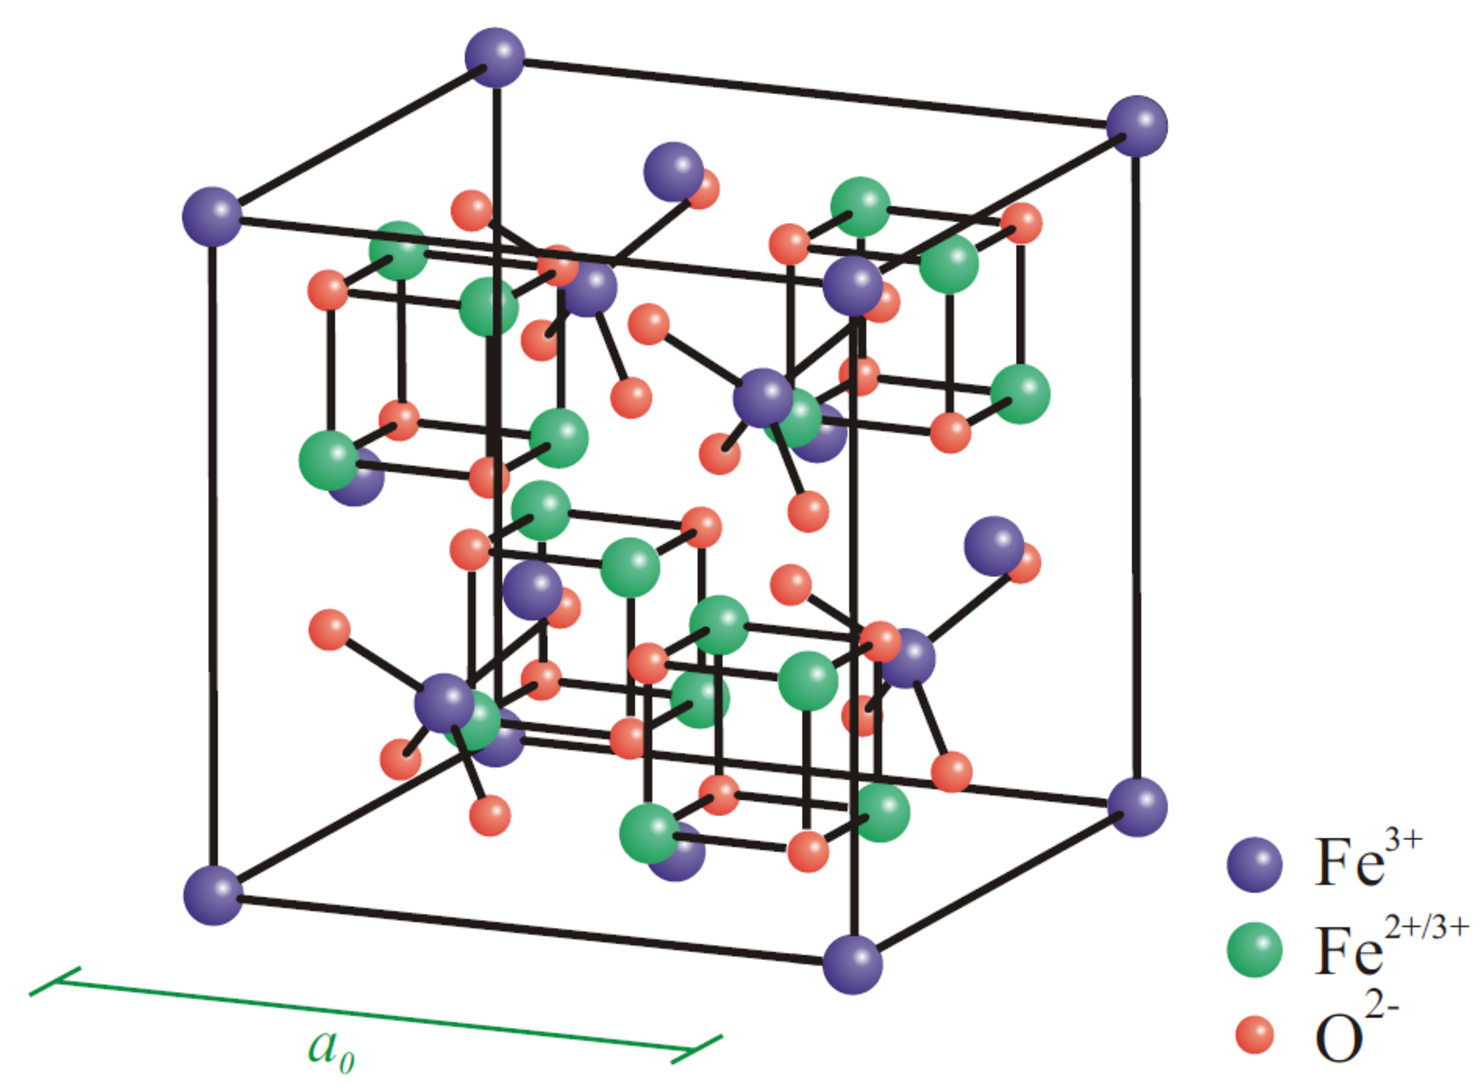
\includegraphics[height=5cm]{Spinell_mod.pdf}
                \caption{Inverse Spinellstruktur von Magnetit.
                Lila sind tetraedrische Plätze zwischen den Sauerstoffatomen dargestellt und in grün oktaedrische Plätze.
                Vorlage aus~\cite{bertram_rontgenstrukturanalyse_2009} und bearbeitet.}
                \label{fig:Spinell}
            \end{figure}
            Magnetit kristallisiert in der in \autoref{fig:Spinell} dargestellten inversen Spinellstruktur, einer kubisch-flächenzentrierten Struktur mit der Gitterkonstanten von \SI{8.397}{\angstrom}~\cite{springer_database}.
            Die Einheitszelle von Magnetit besteht aus zwei $\ce{Fe}^{3+}$ und einem $\ce{Fe}^{2+}$ zu vier $\ce{O}^{2-}$-Ionen.
            Hierbei befinden sich die $\ce{Fe}^{2+}$-Ionen auf $\sfrac{1}{4}$ der oktaedrischen Lücken zwischen den Sauerstoffatomen.
            Dahingegen sitzen die $\ce{Fe}^{3+}$ zu $\sfrac{1}{4}$ auf oktaedrischen Plätzen und zu $\sfrac{1}{8}$ auf tetraedrischen Plätzen.
            Die restlichen $\sfrac{1}{2}$ oktaedrischen und $\sfrac{7}{8}$ tetraedrischen Plätze bleiben frei.

            Die Bandlücke beträgt bei Raumtemperatur nur etwa \SI{0.1}{\electronvolt}~\cite{FeO_23}. %, dabei kommt ein ähnliches Prinzip des Ladungstransfer-Isolators zum Einsatz~\cite{FeO_19}.
            Durch diesen halbmetallischen Charakter weist Magnetit den geringsten elektrischen Widerstand aller Eisenoxide auf~\cite{FeO_23}.
            Interessanterweise unterfährt das Magnetit bei einer Temperatur von \SI{125}{\kelvin} dem Verwey-Übergang und wird zum Isolator.
            Dabei ändert es nicht nur seine elektronischen Eigenschaften, sondern auch die geometrischen, sodass Gitterverzerrungen die Folge sind~\cite{cornell_iron_2003}.
            Die Austrittsarbeit lässt sich auf \SI{5.2}{\electronvolt} bestimmen~\cite{FeO_40}.

            \begin{figure}
                \centering
                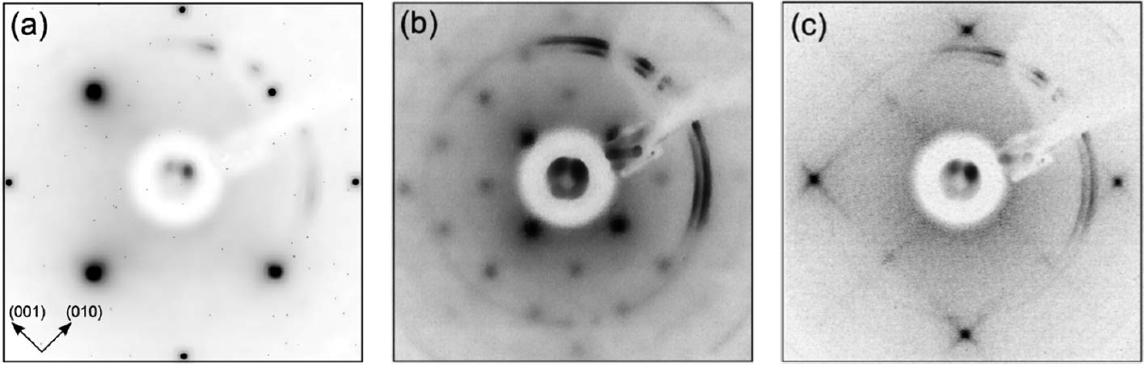
\includegraphics[height=3cm]{LEED_Sub_mod.PNG}
                \caption{Beugung niederenergetischer Elektronen der (001)-Orientierung mit einer Elektronenenergie von \SI{125}{\electronvolt}, (a) eine passivierte Eisenoberfläche, (b) einen \ce{Fe3O4}-Film und (c) für Eisenmonooxid.
                Kopiert aus~\cite{FeO_1} und bearbeitet.}
                \label{fig:LEED_Sub}
            \end{figure}
            In Bezug auf die Oberflächeneinheitszelle des Eisens zeigt die \ce{Fe3O4}-Oberfläche eine nicht rekonstruierte $\text{p}(2\times 2)$ Überstruktur (siehe \autoref{fig:LEED_Sub}(b)). % , da die primitive Einheitszelle der Oberfläche eine Gitterkonstante von \SI{5.9}{\angstrom} besitzt.
            Häufig wird die (100)-orientierte Oberfläche mit einer $(1\times 1)\text{R}\SI{45}{\degree}$ Oberflächeneinheitszelle mit $\sfrac{a}{\sqrt{2}}$ Kantenlänge vorgefunden~\cite{bus_studies_2015}.
            Im Gegensatz zu den anderen Eisenoxiden zeigt die Oberfläche damit eine $\left(\sqrt{2}\times\sqrt{2}\right)\text{R}\SI{45}{\degree}$-Rekonstruktion gegenüber der (100)-Orientierung des Eisens~\cite{ruwisch_vsm-untersuchung_2016}.
            
            Die Curie-Temperatur des ferrimagetischen Halbmetalls Magentit liegt bei \SI{858}{\kelvin}~\cite{nordmann_anfangsstadium_2014}. % Halbmetall da ein Spinkanal isolierend der ander metallisch
            Durch den Ferrimagnetismus bei Raumtemperatur und der damit einhergehenden Magnetisierbarkeit, ist das Material besten für die Anwendung geeignet.
            Besonders interessant wird das Material durch die \SI{100}{\percent}-ige Spinpolarisation nahe der Fermikante.
            So lässt sich theoretisch ein unendlich großer magnetischer Tunnelwiderstand erzielen~\cite{nordmann_anfangsstadium_2014}.
            Heutzutage wird Magnetit schon in Speichermedien, auf Basis von Magnetbändern, eingesetzt ebenso wie zur Katalyse~\cite{zimmermann_epitaktisches_2010}.

        \subsection{Eisenmonooxid} \label{sec:FeO}
            Ebenso wie das Nickeloxid kristallisiert auch das Eisenmonooxid (Wüstit) in der \ce{NaCl}-Struktur~\cite{FeO_4}.
            Dabei beträgt die Gitterkonstante \SI{4.308}{\angstrom}~\cite{springer_database} und die $\ce{Fe}^{2+}$-Ionen befinden sich einer oktaedrischen Position zum Sauerstoff.
            Die $\ce{Fe}^{2+}$-Ionen besitzen dabei sechs Elektronen im d-Niveau und bilden einen \textit{High}-Spin-Zustand.
            Fünf der sechs Spins sind also parallel ausgerichtet und der verbleibende antiparallel, was den größten möglichen Gesamtspin bewirkt~\cite{kupper_electronic_2005}.
            Allerdings ist \ce{FeO} nur oberhalb von \SI{560}{\celsius} stabil.
            Ansonsten handelt es sich um eine nicht-stöchiometrische Verbindung.
            So reduziert sich der Anteil an $\ce{Fe}^{2+}$-Ionen und der Anteil an $\ce{Fe}^{3+}$-Ionen nimmt zu~\cite{FeO_11}.
            Es ergeben sich Defekte im Kationenteilgitter und somit wird von $\ce{Fe}_x\ce{O} (x=\num{0.95}-\num{0.88})$ gesprochen~\cite{Chalkogenide}.
            Die Verbindung kann dabei in Anteile von Magnetit und Eisen übergehen~\cite{parkinson_iron_2016}.
            % Dabei verändert sich die Gitterkonstante, da verschiedene Ionen unterschiedliche Bindungslängen aufweisen.

            Genau wie in Nickeloxid sind beim Eisenmonooxid die (111)-Ebenen untereinander antiferromagnetisch gekoppelt.
            Die Neél-Temperatur liegt mit \SI{198}{\kelvin} allerdings unterhalb der Raumtemperatur~\cite{FeO_4}.
            Die magnetischen Momente der $\ce{Fe}^{2+}$-Ionen sind parallel zu den (111)-Ebenen ausgerichtet, sodass sich auf der (100)-Oberfläche eine abwechselnde Spinausrichtung ergibt.
            Durch die Brechung der Periodizität an der Oberfläche richten sich die magnetischen Momente neu aus.
            In der obersten Lage nehmen diese einen Winkel von \SI{25}{\degree} mit der leichten Achse des Kristalls ([111]) hin zur Oberflächennormalen ein.
            Die inneren Lagen zeigen dabei nur einen Winkel zwischen \SIrange[range-phrase=\:und\:]{4}{8}{\degree} zur leichten Achse~\cite{FeO_6}.
            Als Defekte werden der Eisenmangel in oktaedrischer Umgebung und die Anreicherung von Eisenionen in tetraedrischer Umgebung betrachtet.
            Steigt die Konzentration der Defekte im $\ce{Fe}_x\ce{O}$ an, so steigt ebenfalls die Neél-Temperatur~\cite{FeO_13}.

            Wie schon das \ce{NiO} ist auch \ce{FeO} ein Ladungstransfer-Isolator mit einer Bandlücke von \SI{2.4}{\electronvolt}~\cite{FeO_21} und einer Austrittsarbeit von \SI{3.5}{\electronvolt}~\cite{FeO_28}.
            Mit dieser Energie ist eine Anregung mittels sichtbaren Lichts möglich.
            Anwendung findet dies zum Beispiel bei nanokristallinem Eisenmonooxid als Indikator.
            % Durch die antiferromagnetische Eigenschaft des Eisenmonooxid ist auch dieses für die Anwendung von optoelektrischen Bauteilen prädestiniert, da die Magnonenfrequenz im \si{\tera\hertz}-Bereich liegt.
            Die Schwierigkeit bei Eisenmonooxid besteht darin, eine wohldefinierte und möglichst defektfreie Oberfläche zu erzeugen.
            Hinsichtlich dessen gab es bereits eine Vielzahl an Studien zu Kristallen des FeOs~\cite{FeO_7, FeO_19, FeO_26, FeO_23, FeO_27}.
            % Allerdings mangelt es dabei an Forschung zu dessen Oberflächen~\cite{FeO_1, FeO_4, FeO_29}.
            Entscheidend für die Präparation scheint das Verhältnis aus Sauerstoffdruck und Aufdampfrate des Eisens, ebenso wie die zeitliche Abfolge des Aufheizens der Probe und dessen Temperaturen zu sein.
            Beim Präpartaionsprozess lässt sich über Umwege des Magnetits eine Wüstitstruktur durch Sauerstoff begleitetes Aufdampfen von Eisen auf eine passivierte Eisenoberfläche gewinnen.
            % Bei der Verwendung von passiviertem Eisen als Substrat lässt sich zunächst ein \ce{Fe3O4} Film erzeugen.
            Das Passivieren einer reinen Eisenoberfläche der (100)-Orientierung ergibt das Beugungsbild in \autoref{fig:LEED_Sub}(a).
            Nach dem Aufdampfen des Magnetitfilms ergibt sich das Bild der Beugung von niederenergetischen Elektronen in \autoref{fig:LEED_Sub}(b).
            % Erkennbar ist hier die $\text{p}(2\times 2)$-Überstruktur der kristallterminierten Oberfläche, mit der doppelt so großen Oberflächeneinheitszelle bezüglich des passivierten Eisens mit \SI{2.86}{\angstrom}~\cite{FeO_1}.
            Anschließend geht der Magnetitfilm in Eisenmonooxid über, wenn die Probe bei \SI{800}{\kelvin} ausgeheizt wird~\cite{FeO_1}.
            Was durch die Rekonstruktion sichtbar wird, welche sich in \autoref{fig:LEED_Sub}(c) ergibt.
            Die Intensität ist dabei im Vergleich zum passivierten Eisen invertiert und die Beugungsreflexe sind, auf Grund der größeren primitiven Oberflächeneinheitszelle mit \SI{3.07}{\angstrom}, näher zum Zentrum gerückt~\cite{FeO_1}.
            % Die Reinheit kann mittels Augerelektronenspektroskopie \cite{FeO_1} oder eine genauere Identifizierung mit  Röntgenphotoelektronenspektroskopie des \ce{Fe}3p Signals erfolgen.
            % Dieser enthält einen Anteil für die $\ce{Fe}^{2+}$ und $\ce{Fe}^{3+}$-Ionen~\cite{FeO_7}.

        \subsection{Pentacen} \label{sec:5A}
            Pentacen zeichnet sich durch seine hohen Elektronenmobilität von \SI{3.0}{\centi\meter\squared\volt\per\second} aus und weist damit eine größere Elektronenbeweglichkeit auf als jene des häufig eingesetzten Siliziums mit \SI{1.0}{\centi\meter\squared\volt\per\second}~\cite{5A_13}.
            Seine geringe Größe und die damit verbundenen kleineren möglichen Bauteildimension unterstützt die Anwendungsmöglichkeiten~\cite{IF_15}.
            Mit einer Dichte von nur \SI{1.232(6)}{\gram\per\cubic\centi\meter} ist es besonders leicht, was einen Vorteil für die mobile Anwendungen mit sich bringt~\cite{CAS}.
            Hierdurch wird es bereits als organischer Halbleiter zum Einsatz gebracht~\cite{5A_4}.
            Zum Bespiel in Transistoren \cite{5A_14, 5A_13} und Luftfeuchtigkeitssensoren \cite{demelas_chemical_2015} wird Pentacen heute schon verwendet.
            Diese Bauteile können dann in bestehende Schaltungen eingebaut werden und erhöhen so die Effizienz und können dabei die Baugröße reduzieren, sowie zur Reduktion des Gewichts beitragen.
            % Eine Verwendung in Solarzellen ist ebenfalls denkbar~\cite{shirota_1_2019}.
            % Auf Grund dessen ist eine weitere Erforschung interessant.
  
            \begin{figure}
                \centering
                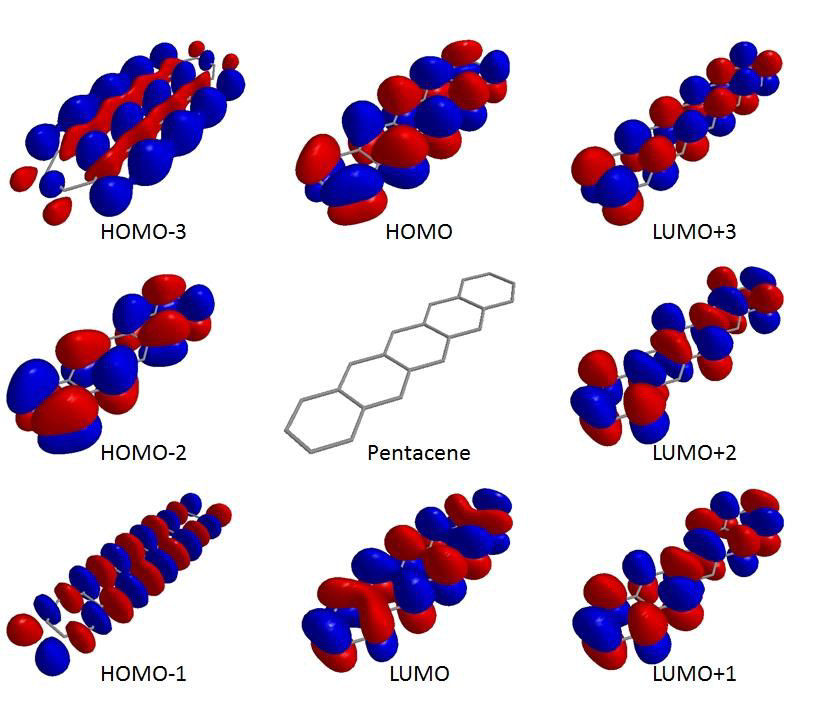
\includegraphics[width=0.6\textwidth]{PEN.jpg}
                \caption{Geometrische Struktur des Pentacen sowie die vier höchsten besetzten und vier niedrigsten unbesetzten Molekülorbitale. Kopiert aus~\cite{PEN}.}
                \label{fig:PEN}
            \end{figure} 
            Bei Pentacen ($\ce{C22H14}$) oder kurz 5A handelt es sich um einen Elektronendonator, der zu den p-Typ Halbleitern gehört~\cite{5A_1}. % Transport wird maßgeblich durch Löcher verursacht.
            Seine Struktur ist in \autoref{fig:PEN} (Mitte) dargestellt, welche sich aus linear an Kanten verschmolzenen Phenylringen zusammensetzt~\cite{MM_2}.
            Ebenfalls zu sehen, sind jeweils die ersten vier höchsten besetzen und niedrigsten unbesetzten Molekülorbitale.
            Dabei konnten diese zuerst mittels Rastertunnelmikroskopie im Jahre 2011 identifiziert werden~\cite{5A_10}.
            Die Elektronen sind in den $\pi_6$-Orbitalen entlang der Phenylringen stark delokalisiert, was zur großen Elektronenbeweglichkeit führt.
            % Dabei weist allerdings Pentacen keinen permanenten Dipol auf~\cite{5A_4}.
       
            Das Molekül Pentacen zeigte bereits auf zahlreichen Oberflächen reproduzierbares Wachstum von dünnen Filmen bei Raumtemperatur \cite{5A_9}.
            Dabei wurden Metalle wie Gold \cite{5A_6}, Silber \cite{5A_4}, Kupfer \cite{5A_1}, Calcium \cite{5A_5} oder dünne Schichten aus Natriumchlorid \cite{5A_10} verwendet.
            Eine bereits häufig verwendete Oberfläche stellt die des Goldes (111) dar.
            Auf ihr ordnen sich die Moleküle wohl definiert an und liegen dabei flach und parallel zum Substrat~\cite{5A_4}.
            % Der Abstand zwischen den Molekülen und Substrat wird auf \SI{3.28}{\angstrom} bestimmt, was in der Größenordnung für Physisorption liegt~\cite{5A_1}.
            % Dabei kamen Techniken wie die Rastertunnelmirkroskopie \cite{5A_7}, Beugung niederenergetischer Elektronen \cite{5A_4}, Rötgenphotoelektronenspektroskopie \cite{5A_5} sowie Photoemissionsorbitaltomographie zum Einsatz.
            % Pentacen bringt die perfekten Eigenschaften für Photoemissionsorbitaltomographie mit, da es sich um ein $\pi$-konjugiertes Molekül handelt~\cite{MM_2}, worauf in \autoref{sec:MOT} genauer eingegangen wird.

            Derzeitige Herausforderungen sind jedoch die Instabilität unter Atmosphäre sowie die Löslichkeit in verschiedenen Lösungsmitteln, welche zur Massenproduktion unabdingbar ist~\cite{kus_chapter_2018}.
            Allerdings zeigten neuste Studien bereits Erfolge, Pentacen aus einer Lösung als dünnen Film aufzubringen~\cite{5A_7}.
            Ein weiterer großer Vorteil des Pentacen ist die einfache Herstellung \cite{kus_chapter_2018} und die Zusammensetzung aus leichten Atomen.
            Für den Einsatz in der Photoemissionsorbitaltomographie (siehe \autoref{sec:MOT}) eignet sich Pentacen aufgrund seiner genannten Eigenschaften.
            % Versuche zur Anordnung von Pentacen auf den \ce{NiO}(111) und \ce{FeO}(100) Oberflächen konnten aktuell noch nicht beobachtet werden.
            % Wohl ist aber bekannt, dass sich Pentacen auf $\ce{Fe}-\text{p}(1 \times 1)\ce{O}$ strukturiert anordnet.